% !TeX spellcheck = cs_CZ
% file: kap_zakld_zakn_elmag.tex
%====================Kapitola: LabVeiw==============================================================
\chapter{LabView}\label{ES:kap_labview}
\minitoc

  \section{Filosofie a součásti vývojového porstředí LabView }
    Základním záměrem vývojových pracovníků firmy National Instruments bylo dát do rukou inženýrů
    nástroj podobné efektivity pružnosti a síly jako je tabulkový procesor v rukou finančního
    manažera. Myšlenka, na níž stojí efektivita vývojového prostředí LabVIEW I daného na trh v roce
    1986 pro platformu počítačů Macintosh je jednoduchá a vznikla původně na půdě Texaské univerzity
    ve skupince nadšenců kolem duchovního `otce tohoto systému Jeffa Kodovského. Vychází se zde z 
    poznatku, že tím, kdo ví, co měřit, jak analyzovat a jak prezentovat data, je technik, který
    nemusí být sám zkušeným programátorem. Své představy tedy předává programátorovi obvykle v
    podobě blokového schématu. Programátor toto schéma potom převádí do syntaxe zvoleného
    programovacího jazyka, což je činnost poměrně zdlouhavá a náročná na přesnost a nepřináší již do
    procesu měření obvykle žádné další nové informace.
     
    \begin{wrapfigure}{r}{8cm}
      \centering
      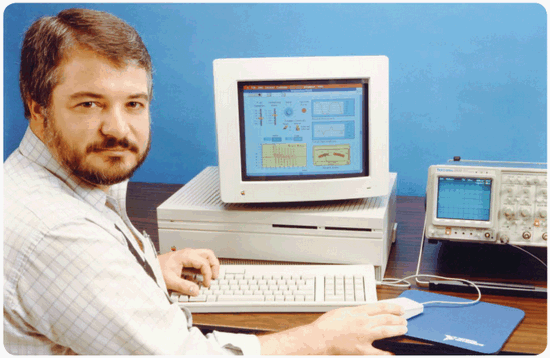
\includegraphics[scale=0.5]{Jeff_Kodovsky_Labview1988.png}
      \caption{Jeff Kodovsky prezentuje ranou verzi programu LabVIEW. Psal se rok 1988. Kredit:
               \niLabviewHistory, \cite{Kodovsky2011}}
      \label{ems:fig_Kodovsky}
   \end{wrapfigure}
    Cílem vývojového prostředí LabVIEW je to, aby blokové schéma bylo koncovým tvarem aplikace,
    který se již dále nebude převádět do textové podoby. LabVIEW (Laboratory Virtual Instruments
    Engineering Workbench) je obecným vývojovým prostředím s bohatými knihovnami pro vytváření
    aplikací zaměřených do oblasti měření ve všech fázích tohoto procesu - tj. sběru, analýzy a
    prezentace naměřených dat. Podporuje všechny čtyři základní způsoby sběru dat do počítače (z
    měřicích přístrojů přes rozhraní RS 232 nebo GPIB, ze zásuvných multifunkčních karet a ze
    systému na bázi VXI sběrnice). Poskytuje uživateli plnohodnotný programovací jazyk se všemi
    odpovídajícími datovými a programovými strukturami v grafické podobě - tzv. G jazyk (Graphical
    language)\cite[p.~21]{Zidek-2002-ID60}.

   LabVIEW je tedy vývojovým prostředím na úrovni např. C jazyka, ale na rozdíl od něj není
   orientován textově, ale graficky.. Výsledný produkt tohoto vývojového prostředí se nazývá
   virtuálním pří- strojem (Virtual Instrument), protože svými projevy a činností připomíná klasický
   přístroj ve své fyzické podobě.
  
   Virtuální přístroj jako základní jednotka aplikace vytvořené v tomto vývojovém prostředí
   obsahuje:
   \begin{itemize}
     \item interaktivní grafické rozhraní (Graphical User Interface - GUI) ke koncovému uživateli -
           tzv. čelní panel (Front Panel), který simuluje čelní panel fyzického přístroje. Obsahuje
           prvky pro ovládání a indikaci (knoflíky, tlačítka, LED indikátory, grafy ..). Tento
           čelní panel ovládá uživatel myší nebo z klávesnice.
     \item činnost virtuálního přístroje je dána jeho blokovým schématem (Block Diagram). Toto
           blokové schéma je vytvořeno ikonami reprezentujícími v koncových blocích ovládací a
           indikační prvky čelního panelu a ve svých uzlových blocích jsou to bloky zpracovávající
           procházející data. Tento blokový diagram je zdrojovou podobou každé aplikace.
     \item virtuální přístroj má hierarchickou a modulární strukturu. Lze jej používat jako celý
           program nebo jeho jednotlivé podprogramy, které se nazývají podřízenými virtuálními
           přístroji (SubVI). Součástí každého virtuálního přístroje je jeho ikona, kterou je
           prezentován v blokovém schématu a konektor s přípojnými místy pro vstupní a výstupní
           signály.         
   \end{itemize}
  
   Těmito charakteristickými rysy naplňuje vývojové prostředí LabVIEW podmínky modulárního
   programování. Svou aplikaci dělí uživatel na jednotlivé úlohy, pro které vytváří dílčí virtuální
   přístroje (subVI) a z nich potom buduje celou aplikaci jejich spojováním do výsledného
   virtuálního přístroje. Na závěr lze celou aplikaci přeložit do EXE tvaru a provozovat nezávisle
   na vývojovém prostředí. Díky možnosti vyzkoušet funkci každého dílčího virtuálního přístroje
   nezávisle na jiných a díky bohaté škále ladicích prostředků je ladění aplikace velmi snadné.
   
 \section{Základní části virtuálního přístroje}
   \subsection{Čelní panel}
   \subsection{Blokové schéma}
   \subsection{Ikona a konektor} 
 \section{Práce s grafy}
   Součástí grafického rozhraní k uživateli tvořeného ve vývojovém prostředí LabVIEW čelním panelem
   virtuálního přístroje jsou velmi často i grafy. Z hlediska dělení objektů čelního panelu na prvky
   ovládací (směr toku informace od uživatele k systému) a indikační (směr toku informace od systému
   k uživateli) se jedná prakticky vždy o objekty indikační. Indikátor grafu tedy představuje
   dvourozměrný displej určený pro zobrazení jednoho nebo více průběhů.
   
   \subsection{Rozdělení grafů}
     Ve vývojovém prostředí LabVIEW lze indikátory grafů zásadně rozdělit podle dvou hledisek:
     \begin{itemize}
       \item podle způsobu předávání dat a zobrazení průběhů v grafu:
         \begin{itemize}
           \item \textbf{statické indikátory} (Graphs), kde pro zobrazení jednoho či více průběhů je
                 nutné předem připravit data popisující celý průběh, popř. průběhy a předat je
                 objektu statického grafu jako celek, graf je zobrazen jednorázově podle zadání dat
                 pro osu nezávisle proměnné se statické grafy dělí na:
              \begin{itemize}
                \item průběhové (časové) grafy (waveform graph), u kterých se předpokládá  
                      rovnoměrné rozdělení bodů tvořících graf na ose x dané počátkem a přírůstkem 
                      - nejčastěji se tento typ grafu používá pro zobrazení časového průběhu 
                      veličiny   
                \item XY grafy (XY graph), u kterých se předpokládá libovolné rozdělení bodů
                      tvořících graf na ose x - s využitím tohoto typu grafu je možno zobrazit
                      libovolný průběh v kartézských souřadnicích
              \end{itemize}  
           \item \textbf{registrační indikátory} (CHARTS), kde vstupní data jsou předávána bod po
                 bodu, popř. jako bloky dat představující úseky zobrazovaného průběhu. Registrační
                 graf postupně doplňuje průběh tak, jak jsou mu dodávána vstupní data.
         \end{itemize}
       \item podle počtu dimenzí grafu:
         \begin{itemize}
           \item grafy dvourozměrné - statické i registrační
           \item grafy třírozměrné zobrazované v ploše - statické i registrační
           \item grafy třírozměrné zobrazované v axonometrickém pohledu s možností natáčení
         \end{itemize}  
     \end{itemize}

     \begin{figure}[ht!]
       \centering
       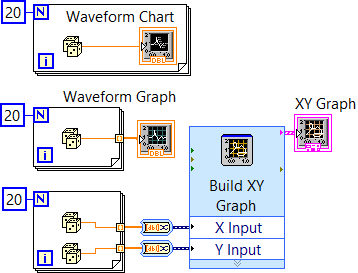
\includegraphics[scale=0.8]{WaveformGraphChartXYd.png} 
       \caption[Waveform Graph, Waveform Chart a XY Graph]{Demonstrace rozdílu mezi registračním
               grafem (Waveform chart) a statickým grafem (Waveform Graph). Pro úplnost je zde
               zastoupen i XY graph.}
       \label{EMS:fig_WaveformGraphChartXYd}
     \end{figure} 
     Jak již bylo řečeno, Waveform Chart se používá pro zobrazení postupně vznikajících průběhů -
     data pro zobrazení jsou na indikátor grafu posílána postupně. Pokud bychom VI z obrázku
     \ref{EMS:fig_WaveformGraphChartXYd} opakovaně spouštěli, byl by vygenerovaný průběh připojen
     na konec předchozího průběhu. Tím by se graf postupně zaplňoval. Při definování tohoto
     typu indikátoru grafu je vhodné aby uživatel mimo jiné určil:
     \begin{itemize}
       \item šířku zobrazovaného průběhu v počtu bodů - lze si to představit jako okno dané šířky,
             přes které se dívám na zobrazovaný průběh – zadává se jako dolní a horní mez při popisu
             osy x
       \item šířku zapamatované části grafu v počtu bodů, která je obvykle větší než šířka
             zobrazovaného průběhu a umožňuje mi tak podívat se i na starší data, která se nevejdou
             do zobrazované části průběhu – zadává se přes roletové menu v položce Chart History
             Length. 
     \end{itemize}
     
   \subsection{Datové struktury pro indikátory grafů}
     Podle zvoleného typu grafu je nutno pro něj připravit i vhodnou datovou strukturu odpovídající
     vybranému typu grafu a počtu požadovaných průběhů v něm zobrazených. V následujícím popisu
     datových struktur je použita tato konvence:
     \begin{itemize}
       \item \([y]\) představuje jednorozměrné pole prvků \(y\)
       \item \({y1,y2,y3}\) představuje cluster s prvky \(y1\),\(y2\) a \(y3\) 
     \end{itemize} 
     Pro programové vytvoření odpovídajících datových struktur se používá:
     \begin{itemize}
       \item v případě pole funkce Build Array nebo zapnutá indexace na výstupu z programových
             struktur cyklu typu FOR a typu WHILE. 
       \item v případě clusteru funkce Bundle eventuálně funkce Bundle by Name
     \end{itemize}

     V případě složitějších datových struktur se tyto funkce kombinují, přičemž se postupuje od
     středu definice datové struktury k okrajům.  
       
     \begin{figure}[ht!]
       \centering
       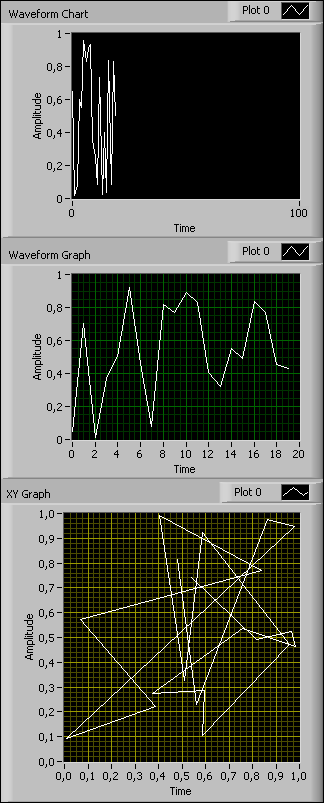
\includegraphics[scale=0.8]{WaveformGraphChartXYp.png} 
       \caption[Waveform Graph, Waveform Chart a XY Graph]{Demonstrace rozdílu mezi registračním
       grafem (Waveform chart) a statickým grafem (Waveform Graph). Pro úplnost je zde zastoupen i
               XY graph}
       \label{EMS:fig_WaveformGraphChartXYp}
     \end{figure} 
        
%---------------------------------------------------------------------------------------------------
\printbibliography[title={Seznam literatury},heading=subbibliography]
\addcontentsline{toc}{section}{Seznam literatury}
